\documentclass[border=4pt]{standalone}
\usepackage{tikz}
\usetikzlibrary{arrows.meta,calc,shapes.geometric}

\begin{document}
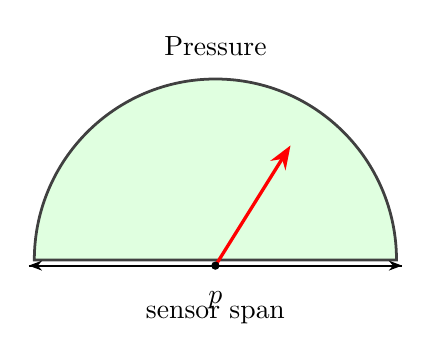
\begin{tikzpicture}[>=Stealth]
  \node[semicircle,draw=black!75,fill=green!12,line width=1pt,
    minimum width=46mm,minimum height=23mm,outer sep=2pt] (gauge) at (0,0) {};
  \coordinate (pivot) at (gauge.chord center);
  \draw[thick] (gauge.arc end) -- (gauge.arc start);
  \draw[red,-{Stealth[length=3mm]},line width=1.2pt]
    (pivot) -- ($(pivot)!18mm!58:(gauge.arc start)$);
  \fill (pivot) circle (1.5pt);
  \node[below=2mm] at (pivot) {$p$};
  \node[above=1mm] at (gauge.apex) {Pressure};
  \draw[<->] (gauge.arc end) -- node[below=4mm] {sensor span} (gauge.arc start);
\end{tikzpicture}
\end{document}
